\section{The broadcast operation is a one-to-all collective communication operation where
one of the processes sends the same message to all other processes.}
\subsection{Design an algorithm for the broadcast operation using only point-to-point communications which requires only $O(log P)$ communication steps}
The following figure describes the steps of our algorithm. The showcase uses $P = 2^D$, but the algorithm is functional for any P.
\begin{figure}[H]
\centering
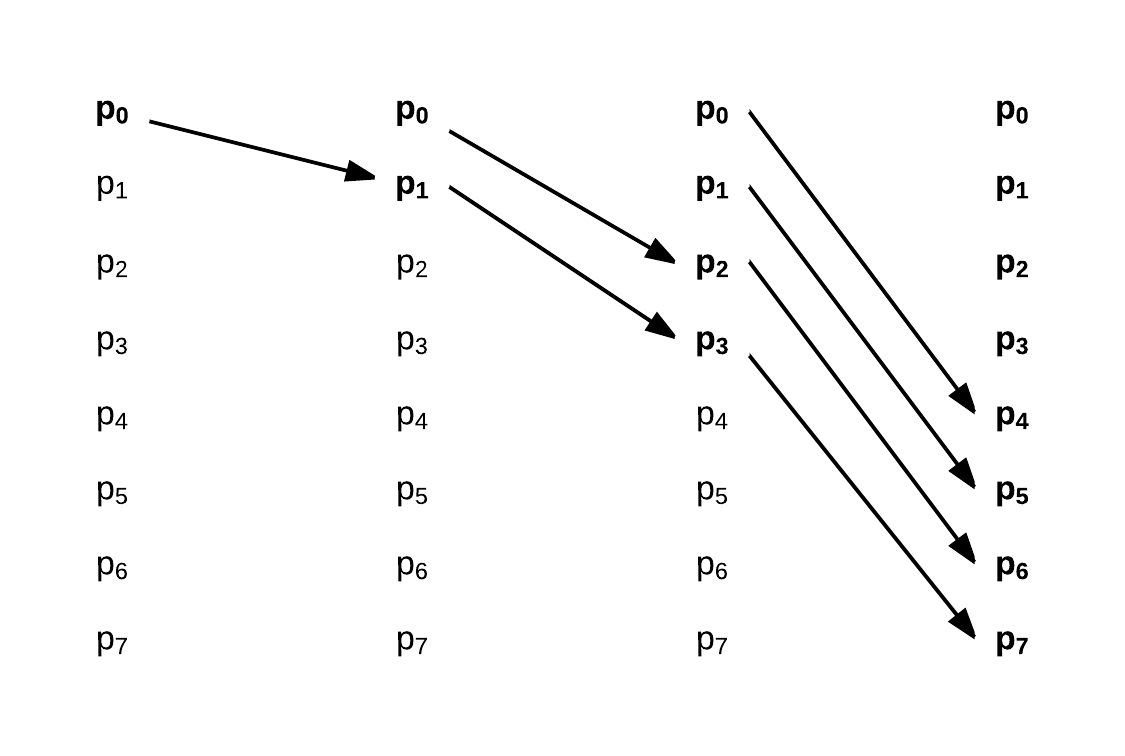
\includegraphics[width=0.7\linewidth]{img/communication_propagation.png}
\caption{Communication broadcast algorithm in $O(log P)$}
\end{figure}

This figure illustrates the following algorithm. For any \textit{p} higher than 0, the process will receive its message from $p_{sender} = p_{receiver} - 2^D$ with \textit{D} such that $2^D \leq p_{receiver} \leq 2^{D+1} $.

\begin{algorithmic}
\If{p == 0}
    \State D = 0
    \State msg = "message"
\Else
    \State D = trunc($log_2(p)$)
    \State msg = receive($p - 2^D$)
    \State ++D
\EndIf
\State 
\While{$p + 2^D \le p$}
    \State send(msg, $p + 2^D$)
    \State ++D
\EndWhile
\end{algorithmic}


\subsection{Do a (time-)performance analysis for your algorithm}
The process involves no computation on any processor. We denote the communication time required to send the data set, consisting of $n$ elements, between two processors $t_{comm}$. As usual $t_{comm} =t_{startup}+nt_{data}$. Each step in the algorithm takes time $t_{comm}$, in total $D=\log_2{P}$ steps are required. Altogether this yields the total time as a function of $P$ and $n$ as: 

\[T = (t_{startup}+nt_{data} )\cdot \log_2{P}   \]

\subsection{How can the scatter operation be implemented using $O(logP)$ communication steps?}
Suppose we have a data set consisting of $P$ elements known by a process $p_0$. We want to scatter the data so that a process $i$ holds one element of the data set, also named element $i$. We would do this using the broadcast algorithm previously defined, replacing some calls by the following:

\begin{algorithmic}
\If{p == 0}
    \State D = 0 size
    \State data = loadData()
\Else
    \State D = trunc($log_2(p)$) \Comment{cast from double to int}
    \State data = receive($p - 2^D$)
    \State ++D
\EndIf
\State 
\While{$p + 2^D \le p$}
    \State array = split(data, 2) \Comment{Split the dataset in two parts of equal size}
    \State data = array[0]
    \State send(array[1], $p + 2^D$)
    \State ++D
\EndWhile
\end{algorithmic}

After the first iteration, two processes will each hold one half of the data. After 2 iterations 4 processors hold one fourth each, and so forth until all $P$ processors hold exactly one element. The number of iterations is:

\[ D = \frac{\log(P)}{\log(2)} \Rightarrow T \propto \log_2(P) \]

\section{Consider a matrix A distributed on a $P*P$ process mesh. An algorithm has been given in the lecture for evaluating the matrix-vector product $y = Ax$. While x is column distributed, y is row distributed. In order to carry out a further multiplication Ay, the vector y must be transposed.}
\subsection{Design an algorithm for this transposition. You may use the results from
problem 1.}

In order to perform the transposition of the vector \textit{y}, two steps are necessary (if we consider the current state as the one immediately after the internal multiplication of $x_c$ by $A_{r,c}$ by $p_{r,c}$). We consider here that \textit{A} is a square matrix (since we juste performed the $Ax$ operation and want to perform $Ay$) which is distributed on the $P*P$ mesh grid. We also assume that $P = M$, with A a matrix of $M*M$.

\begin{figure}[H]
\centering
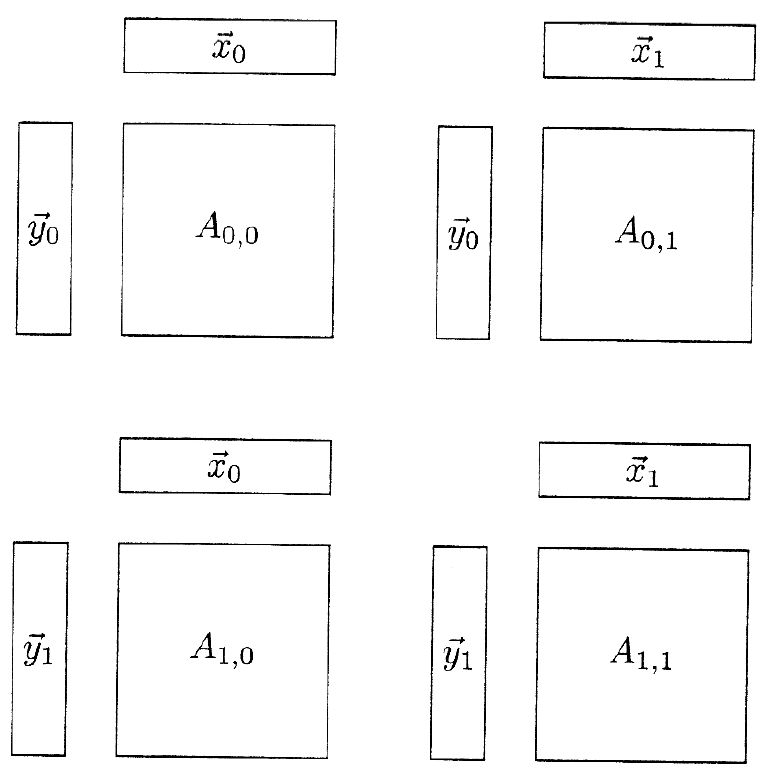
\includegraphics[width=0.7\linewidth]{img/matrix_multi.jpg}
\caption{Data distribution for each processor, with A a square matrix}
\end{figure}

Therefore, our transition algorithm would first require an efficient information exchange between the processes of the same row to compute $y_r$ (this should be achived using recursive doubling with a complexity of $O(log P)$ for the whole matrix), then an axial symmetry communication to achieve the final transposition (we assume that each process knows its row \textit{r} and column \textit{c}).

Let $2^D < P < 2^{D+1}$

\begin{algorithmic}
\State s = $y_r$ \Comment{$y_r$ is still incomplete and is only a part of the real $y_r$}
\If{$p \geq 2^D$}
    \State send(s, bitflip(p, $p_{r,D}$))
\EndIf
\If{$p \le P-2^D$}
    \State receive(h, bitflip(p, $p_{r,D}$))
    \State $s = s + h$
\EndIf
\If{$p \le 2^D$}
    \For{d = 0:D-1}
        \State send(s, bitflip(p, $p_{r,D}$))
        \State receive(h, bitflip(p, $p_{r,D}$))
        \State s = s+h
    \EndFor
\EndIf
\If{$p \le P-2^D$}
    \State send(s, bitflip(p, $p_{r,D}$))
\EndIf
\If{$p \geq 2^D$}
    \State receive(s, bitflip(p, $p_{r,D}$))
\EndIf
\State $y_r$ = s \Comment{$y_r$ has now been summed and is known by every process of the same row}
\If{r != c} \Comment{No permutation required if the process is on the diagonal}
    \State MPI\_Sendrecv($y_r$, $p_{c,r}$, $y_c$, $p_{c,r}$) \Comment{$y_r$ is sent and we retrieve $y_r$}
\EndIf
\end{algorithmic}

On the other hand, if we do not have a vector to sum and transpose but a square matrix of size PxP distributed on a PxP mesh grid, the algorithm is the following:

\begin{algorithmic}
\If{r != c} \Comment{No permutation required if the process is on the diagonal}
    \State MPI\_Sendrecv($y_r$, $p_{c,r}$, $y_c$, $p_{c,r}$) \Comment{$y_r$ is sent and we retrieve $y_r$}
\EndIf
\end{algorithmic}

\subsection{Make a performance analysis}
The complexity of the first algorithm (summing the parts ov the vector $\vec{y}$ then applying a transposition to prepare the system for the multiplication $yA$) is $O(log(P) + 2)$.

The complexity of the second algorithm for a square matrix is O(1).


\section{Parallel implementation of the Jacobi iteration}
\textit{See the following pages.}
